% !TEX program = xelatex
% Group meeting slides. Compile with XeLaTeX, twice.
% Content source: paper/main.tex, SHA256 EF7421988ED2194163A25A4281273404A2E0487AD817F2F19EDDE8310D43A726
% Introduction source: E:/YTT/GROUP/DynFL-reconfiguration/tex/paper/main.tex, SHA256 B90F48AD7307E4990A01BDF02BF5C62B284E6B8CA2B6F6BFDD17D516FFD8D192
\documentclass[aspectratio=169,11pt]{beamer}
\usepackage[UTF8,fontset=fandol]{ctex}
\usepackage{amsmath,amssymb,booktabs,array,graphicx,colortbl}
\usepackage{tikz}
\usetikzlibrary{arrows.meta,positioning,calc}
\usepackage{pgfpages}
\setbeameroption{hide notes}
% For a presenter display, replace the preceding line with:
% \setbeameroption{show notes on second screen=right}
\definecolor{Navy}{HTML}{15344D}
\definecolor{Teal}{HTML}{00857D}
\definecolor{Orange}{HTML}{D87730}
\definecolor{Gray}{HTML}{52616D}
\definecolor{Light}{HTML}{E8EFF3}
\definecolor{Pale}{HTML}{F3F7F8}
\setbeamercolor{normal text}{fg=Navy,bg=white}
\setbeamercolor{structure}{fg=Teal}
\setbeamercolor{frametitle}{fg=Navy,bg=white}
\setbeamercolor{alerted text}{fg=Orange}
\setbeamercolor{item}{fg=Teal}
\setbeamerfont{frametitle}{size=\Large,series=\bfseries}
\setbeamerfont{title}{size=\LARGE,series=\bfseries}
\setbeamertemplate{navigation symbols}{}
\setbeamertemplate{itemize item}{\raisebox{.15ex}{\scriptsize$\bullet$}}
\setbeamertemplate{itemize subitem}{\scriptsize--}
\setbeamersize{text margin left=.75cm,text margin right=.75cm}
\setbeamertemplate{frametitle}{\vspace{.18cm}\insertframetitle\par\vspace{.06cm}{\color{Teal}\hrule height 1.1pt}\vspace{.12cm}}
\setbeamertemplate{footline}{\hspace{.75cm}\raisebox{.16cm}{\color{Gray}\fontsize{7.5}{9}\selectfont 杨婷婷\quad 课题组汇报\hspace{8cm}\insertframenumber}\vspace{.08cm}}
\newcommand{\FlE}{\mathrm{FL}_{E}}
\newcommand{\FlEC}{\mathrm{FL}_{EC}}
\newcommand{\FlC}{\mathrm{FL}_{C}}
\newcommand{\key}[1]{{\color{Teal}\bfseries #1}}
\newcommand{\src}[1]{\vfill{\color{Gray}\fontsize{7.5}{9}\selectfont 依据：#1\par}}
\newcommand{\msg}[1]{\par\vspace{.14cm}{\color{Teal}\rule{.32cm}{1.5pt}}\hspace{.18cm}\textbf{#1}\par}
\newcommand{\figfit}[3]{\includegraphics[width=#1,height=#2,keepaspectratio]{#3}}
\newcommand{\tight}{\setlength{\itemsep}{.18cm}}
\graphicspath{{assets/}}
\title{层次化联邦学习中的\\动态协作模式选择}
\subtitle{近两周工作汇报}
\author{杨婷婷\quad Tingting Yang}
\institute{北京邮电大学\quad 数学科学学院}
\date{2026年10月26日}
\begin{document}

% 01
\begin{frame}[plain]
\par\vspace{.5cm}
{\color{Teal}\rule{1.0cm}{2.5pt}}\par\vspace{.45cm}
{\LARGE\bfseries 层次化联邦学习中的\\[.18cm]动态协作模式选择\par}
\par\vspace{.35cm}
{\small Dynamic Collaboration Mode Selection\\in Hierarchical Federated Learning\par}
\par\vspace{.55cm}
{\large 近两周工作汇报\par}
\par\vspace{.22cm}
从七模式联合误差建模，到三模式历史更新评分
\vfill
杨婷婷\quad Tingting Yang\hfill 2026年10月26日\par
\par\vspace{.12cm}
{\small 北京邮电大学\quad 数学科学学院}
\note{本次先介绍研究过程：起初在含split的七模式中联合考虑隐私、学习与效率；由于选择前直接评价联合学习误差存在信息依赖，本阶段聚焦三种非split模式，并重构为历史更新偏差选择信号。之后汇报当前建模和实验。七模式稿用于说明初始设想，当前三模式稿提供后续实验结果。主体约27分钟，附录页用于回答问题。}
\end{frame}

% 02
\begin{frame}{近两周完成的工作}
\renewcommand{\arraystretch}{1.7}
\begin{tabular}{@{}p{.6cm}p{3.15cm}p{9.0cm}@{}}
\key{01} & \textbf{收敛研究范围} & 从七模式误差建模，转向三种非split模式的历史更新评分。\\
\key{02} & \textbf{建立历史更新评分} & 按模式维护历史偏差，用候选聚合单元的样本权重组合成 $J$。\\
\key{03} & \textbf{实现有限候选选择} & 将 $J$ 与估计时延归一化，比较 Greedy、迟滞和周期控制。\\
\key{04} & \textbf{形成实验与解释闭环} & 完成45次主实验的结果整理，并分析训练量、通信与切换成本。\\
\end{tabular}\par
\msg{工作主线：定义可选模式 → 构造选择信号 → 实验验证与结果解释}
\src{当前论文第1、3、4、5节}
\note{这页先回答本阶段做了什么。第一项是问题与边界，第二项是评分的具体构造，第三项是能执行的选择流程，第四项是实验矩阵与结果解释。45次主实验是15种策略、3个随机种子的组合；短期pilot另计。不要把这些工作讲成已完成物理部署。}
\end{frame}

% Research background, added before the research problem.
\begin{frame}{研究背景：三种联邦学习架构}
\begin{columns}[c,onlytextwidth]
\begin{column}{.64\textwidth}
\centering
\figfit{\linewidth}{5.65cm}{federated_learning_architectures.png}
\end{column}
\begin{column}{.32\textwidth}
\key{云端联邦学习}\par
客户端本地训练，更新直接汇聚到云端。
\par\vspace{.30cm}
\key{边缘联邦学习}\par
客户端与Edge协作，由Edge完成聚合。
\par\vspace{.30cm}
\key{层次化联邦学习}\par
先在Edge聚合，再由Cloud进行跨Edge聚合。
\end{column}
\end{columns}
\msg{本研究关注：层次化系统中的动态协作模式选择}
\src{联邦学习架构示意}
\note{配图由用户提供，文件为assets/federated_learning_architectures.png，原始文献来源未提供。依次说明云端、边缘与层次化架构，随后聚焦右侧的层次化协作。图中是三类系统架构；论文的FL_E、FL_EC、FL_C则是同一云—边—端系统内的三种协作方式，不应逐项对应。}
\end{frame}

% Research trajectory: the seven-mode proposal motivates the current study.
\begin{frame}{初始目标：协调隐私、学习表现与效率}
\begin{columns}[T,onlytextwidth]
\begin{column}{.49\textwidth}
\key{七模式协作重配置设想}
\begin{itemize}\tight
\item 同时考虑本地完整训练与跨层split训练。
\item 改变执行位置、传输对象与聚合路径。
\item 根据暴露信息考虑DP与HE保护。
\end{itemize}
\par\vspace{.20cm}
希望解释不同协作与保护配置如何影响学习更新及系统代价。
\end{column}
\begin{column}{.46\textwidth}
\key{含split训练的4种模式}
\[
\begin{gathered}
\mathrm{LIE},\quad\mathrm{LIC},\\
\mathrm{LIEIIC},\quad\mathrm{LIEIIIC}
\end{gathered}
\]
\par\vspace{.15cm}
\key{完整本地训练的3种模式}
\[
\mathrm{LIIE},\quad\mathrm{LIIC},\quad\mathrm{LIIEIIIC}
\]
\end{column}
\end{columns}
\msg{原方案以学习误差和时延为双目标，隐私与资源作为约束}
\src{七模式稿：Model Construction与Global Multiobjective Collaborative Optimization；研究动机结合作者说明}
\note{依据E:/YTT/GROUP/DynFL-reconfiguration/tex/paper/main.tex。最初研究希望协调隐私、学习和效率，但稿件正式优化的是学习误差与时延，隐私属于可行性约束。这里展示的是初始研究范围，不把其中的HE、split训练或七模式实验当作当前三模式方法已经完成的内容。}
\end{frame}

\begin{frame}{关键困难：选择前如何评价联合学习误差}
\[
\begin{aligned}
J_{\mathrm{learn}}^t
&=\mathbb E_t\|\Delta_s^t-\Delta_*^t\|_2^2\\
&=\|e_{\mathrm{alg}}^t+e_{\mathrm{agg}}^t+b_s^t\|_2^2
+\operatorname{Tr}(V_s^t)
\end{aligned}
\]
\begin{itemize}\setlength{\itemsep}{.14cm}
\item \textbf{无保护的反事实更新 $u_{i,0}^t$}：同一候选配置下，无隐私保护时的更新参考。
\item \textbf{理想梯度步 $\Delta_*^t=-\eta_t\nabla F(w^t)$}：需要全局梯度参考。
\item \textbf{扰动均值与协方差}：需要刻画加噪训练轨迹相对参考的统计差异。
\end{itemize}
\par\vspace{.10cm}
{\small 旧稿主文采用clean/private配对校准；附录另有依赖额外假设的在线上界。}
\msg{仅靠一次实际DP执行，难以直接得到候选的精确误差}
\src{七模式稿：Joint Learning Error Modeling与Pre-decision online learning-error bound}
\note{依据七模式稿eq:j_learn_exact及其后校准段。J_learn越小越好。障碍是在线选择前对各候选进行直接、精确且可靠的评价，不是缺少数学定义或任何计算方案。旧稿已有配对clean/private校准表和附条件在线上界；后者需要有效梯度界、稳定性常数及完整噪声模型，不能仅凭这些公式宣称已对全部七模式实现并验证。研究调整的动因由作者本次说明提供。}
\end{frame}

\begin{frame}{本阶段调整：三种非split模式与历史选择信号}
\begin{columns}[T,onlytextwidth]
\begin{column}{.45\textwidth}
\key{研究范围收敛}
\[
\mathcal H=\{\FlE,\FlEC,\FlC\}
\]
\begin{itemize}\tight
\item 在客户端执行完整本地训练。
\item 保留不同聚合路径及训练阶段。
\item 保留DP与生命周期预算约束。
\end{itemize}
\end{column}
\begin{column}{.51\textwidth}
\key{选择依据重构}
\[
d_k^\tau=u_{k,\mathrm{DP}}^\tau-v_g^{\tau-1}
\]
\begin{itemize}\tight
\item 以DP历史更新估计模式偏差。
\item 更新综合反映训练、数据、路径与保护机制的作用。
\item 历史评分 $J$ 偏好较大信号，$J_{\mathrm{learn}}$ 偏好较小误差。
\end{itemize}
\end{column}
\end{columns}
\par\vspace{.22cm}
\key{当前研究定位}\par
在资源与生命周期隐私约束下，用历史更新信号指导动态协作，\\
研究学习表现与系统时延之间的折中。
\src{当前三模式稿第3.3.2节与Discussion；研究范围调整结合作者说明}
\note{本页是研究路线的关键转折。三模式保留原完整本地训练类结构，但不是对旧模式简单改名：当前FL_E还明确包含异步Cloud转发。v_g是历史Cloud聚合更新的EMA，不是直接观测的理想梯度。历史评分间接保留DP保护对更新特征的影响，并未单独分离噪声效应，也不是旧J_learn的估计器。当前实验不建立隐私、精度与效率三个变量的联合最优前沿。}
\end{frame}

% 03
\begin{frame}{研究问题：固定协作分配难适应异构条件}
\begin{columns}[T,onlytextwidth]
\begin{column}{.49\textwidth}
\centering
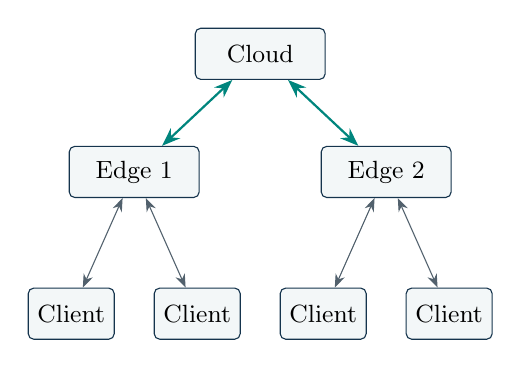
\begin{tikzpicture}[>=Stealth, every node/.style={font=\small},tier/.style={draw=Navy,rounded corners=2pt,minimum width=1.65cm,minimum height=.65cm,fill=Pale}]
\node[tier] (c) at (0,3.3) {Cloud};
\node[tier] (e1) at (-1.6,1.8) {Edge 1};
\node[tier] (e2) at (1.6,1.8) {Edge 2};
\node[tier,minimum width=.9cm] (l1) at (-2.4,0) {Client};
\node[tier,minimum width=.9cm] (l2) at (-.8,0) {Client};
\node[tier,minimum width=.9cm] (l3) at (.8,0) {Client};
\node[tier,minimum width=.9cm] (l4) at (2.4,0) {Client};
\draw[<->,thick,Teal] (c)--(e1);
\draw[<->,thick,Teal] (c)--(e2);
\foreach \a/\b in {l1/e1,l2/e1,l3/e2,l4/e2}{\draw[<->,Gray] (\a)--(\b);}
\end{tikzpicture}
\end{column}
\begin{column}{.47\textwidth}
\begin{itemize}\tight
\item \textbf{数据异构}：不同客户端的更新方向可能不同。
\item \textbf{系统异构}：计算和内存存在异构，链路条件随轮次变化。
\item \textbf{选择问题}：本轮应将多少客户端分配到哪种协作模式？
\end{itemize}
\par\vspace{.25cm}
\key{希望观察的关系}\par
历史更新特征、系统时延与后续学习表现之间如何取舍？
\end{column}
\end{columns}
\src{论文引言与系统模型；图为汇报用的架构示意}
\note{可以用一个直观例子解释：同样一套模式比例，在链路较好和链路较差的轮次，代价可能不同；多进行边缘阶段也会增加训练量。因此需要比较可行分配。当前数据仍保留在客户端，Edge承担聚合；不要将本稿讲成把神经网络分割到远端训练。}
\end{frame}

% 04
\begin{frame}{本阶段的研究切入点}
\renewcommand{\arraystretch}{1.45}
\begin{tabular}{@{}p{3.0cm}p{4.4cm}p{5.0cm}@{}}
\toprule
\textbf{已有研究方向} & \textbf{关注的问题} & \textbf{本阶段选择的切入点}\\
\midrule
异构HFL & 资源管理、模型适配、聚合控制 & 在三种协作模式之间选择客户端分配\\
多层协作 & 跨层训练、聚合与同步机制 & 用有限候选表示不同协作分布\\
隐私保护 & DP机制、预算管理与保护策略 & 将生命周期预算纳入候选可行性\\
\bottomrule
\end{tabular}\par
\par\vspace{.35cm}
\key{本稿的具体方法}\par\vspace{.15cm}
把模式相关的历史更新偏差与候选的聚合结构联系起来，\\
再结合估计系统时延，形成可执行的选择准则。
\src{论文第2节与第1节贡献概述}
\note{这页用于交代定位，不主张之前的所有方法都只能用固定结构。已有方法已经覆盖自适应聚合、资源调度和多种隐私机制。本阶段的具体设计是三模式分布、历史评分与系统代价的结合。DP-SGD和RDP是采用的现有技术。}
\end{frame}

% 05
\begin{frame}{三种模式改变聚合路径与训练阶段}
\renewcommand{\arraystretch}{1.6}
\begin{tabular}{@{}p{1.35cm}p{8.8cm}p{2.2cm}@{}}
\toprule
\textbf{模式} & \textbf{流程} & \textbf{实验训练量}\\
\midrule
$\FlE$ & 本地训练 → Edge聚合；Edge模型返回客户端，更新向Cloud传播 & 1阶段 $\times$ 2步\\
$\FlEC$ & 本地训练与Edge聚合重复 $E_B$ 次，再向Cloud提交最终更新 & 3阶段 $\times$ 2步\\
$\FlC$ & 本地训练后，直接向Cloud提交更新 & 1阶段 $\times$ 2步\\
\bottomrule
\end{tabular}\par
\par\vspace{.25cm}
\begin{itemize}\tight
\item 数据始终保留在客户端；本地训练使用DP-SGD。
\item 同一轮中，不同客户端可以采用不同模式。
\item 多阶段模式同时改变聚合过程与实际训练工作量。
\end{itemize}
\src{论文第3.1节，实验配置表2}
\note{先讲每种模式做了什么，再谈选择。FL_E在Edge形成模型后返回客户端，同时对Cloud作贡献。FL_EC在本轮有3个本地训练与边缘聚合阶段，FL_C直接上传。可用三种模式不同的训练阶段数说明后续训练工作量的差异。}
\end{frame}

% 06
\begin{frame}{用5个候选分布表示可选择的客户端分配}
\begin{columns}[T,onlytextwidth]
\begin{column}{.58\textwidth}
\renewcommand{\arraystretch}{1.45}
\centering
\begin{tabular}{lrrrr}
\toprule
候选 & $\FlE$ & $\FlEC$ & $\FlC$ & 步数/轮\\
\midrule
$P_0$ &30\%&30\%&40\%&320\\
$P_1$ &50\%&25\%&25\%&300\\
\rowcolor{Pale}
$P_2$ &25\%&50\%&25\%&400\\
$P_3$ &25\%&25\%&50\%&300\\
$P_4$ &40\%&40\%&20\%&360\\
\bottomrule
\end{tabular}\par
\end{column}
\begin{column}{.38\textwidth}
\textbf{每个候选先构造成实际分配}
\begin{itemize}\tight
\item 按Edge生成整数客户端配额。
\item 检查资源、隐私和系统准入。
\item 只比较当轮可行的候选。
\end{itemize}
\par\vspace{.2cm}
\key{每次最多评价 $M=5$ 个候选。}
\end{column}
\end{columns}
\par\vspace{.25cm}
标称比例经整数分配与调整；“步数/轮”是全体客户端本地训练步数之和。
\src{论文第3.4节与第5.3.1节}
\note{候选并不等于搜索所有客户端组合。5个候选是一个受控的决策空间，便于检查偏好和成本。P2给FL_EC的比例最高，因此每轮总本地训练步数也最多。这里的O(M)只指候选评估次数，单个候选的分配、时延和向量评分仍有计算成本。}
\end{frame}

% Cloud update units: definition, reassignment, and sample weights.
\begin{frame}{云更新单元：Cloud实际聚合的更新对象}
\textbf{Cloud将每份被接纳的更新作为一个聚合单元 $k$。}
\par\vspace{.25cm}
\renewcommand{\arraystretch}{1.5}
\begin{tabular}{@{}p{1.4cm}p{4.8cm}p{6.4cm}@{}}
\toprule
\textbf{模式} & \textbf{单元对应的客户端} & \textbf{提交给Cloud的对象}\\
\midrule
$\FlE$ & 同一Edge中的该模式客户端组 & Edge聚合更新；异步发送，在接纳它的Cloud聚合中计入\\
$\FlEC$ & 同一Edge中的该模式客户端组 & 完成 $E_B$ 阶段后的最终Edge更新\\
$\FlC$ & 每个客户端各自形成一个单元 & 该客户端直接提交的更新\\
\bottomrule
\end{tabular}\par
\par\vspace{.20cm}
$\mathcal K^t(\mathbf h^t)$：本次Cloud聚合纳入的单元集合。\par
$m(k)$：单元 $k$ 对应的协作模式。
\src{论文第3.3.2节：Cloud aggregation and weights}
\note{先区分客户端和云更新单元：客户端是训练参与者，单元是Cloud看到的聚合输入。Edge聚合路径把同Edge同模式的客户端组合成一份更新；FL_C客户端仍逐个形成单元，即使它们关联同一个Edge。FL_E只在接受其异步更新的Cloud聚合中计入。K依赖当前模式分配和被接纳的更新集合。}
\end{frame}

\begin{frame}{模式切换改变云更新单元的组成}
\begin{columns}[T,onlytextwidth]
\begin{column}{.48\textwidth}
\centering
\key{切换前：6个单元}\par\vspace{.08cm}
\figfit{\linewidth}{4.5cm}{client_mode_grouping_a.png}
\end{column}
\begin{column}{.48\textwidth}
\centering
\key{切换后：7个单元}\par\vspace{.08cm}
\figfit{\linewidth}{4.5cm}{client_mode_grouping_b.png}
\end{column}
\end{columns}
\par\vspace{.12cm}
\begin{itemize}\setlength{\itemsep}{.08cm}
\item $l_2:\FlEC\to\FlC$，从Edge组移出，独立形成Cloud更新单元。
\item $l_5:\FlE\to\FlEC$，与 $l_1$ 组成新的 $\FlEC$ 单元。
\end{itemize}
\src{论文第3.3.2节分组示意图；$k_i$在各轮分别编号，同名不表示固定客户端组}
\note{结合两张原图说明：切换前的k1代表l1、l2，切换后的k1代表l1、l5，而l2成为独立的k2。编号在各轮分别定义，因此不能把跨轮的k1理解为同一个固定组。示例中的单元数由6变7，反映聚合输入结构的改变；单元数本身不等同于学习收益。}
\end{frame}

\begin{frame}{单元样本权重如何接入历史评分}
\begin{columns}[T,onlytextwidth]
\begin{column}{.54\textwidth}
\key{权重由单元代表的样本数确定}
\[
N_k^t=\sum_{i\in\mathcal M_k^t}n_i
\]
\[
\boxed{\quad I_k^t(\mathbf h^t)
=\frac{N_k^t}
{\sum_{\ell\in\mathcal K^t(\mathbf h^t)}N_\ell^t}\quad}
\]
\small
$\mathcal M_k^t$：单元 $k$ 代表的客户端。\par
$n_i$：客户端 $i$ 的训练样本数。\par
分母统计本次被接纳单元代表的总样本数。
\end{column}
\begin{column}{.42\textwidth}
\key{对应前后分组示例}
\[
N_{k_1}^{t-1}=n_1+n_2
\]
\[
N_{k_1}^{t}=n_1+n_5,\qquad N_{k_2}^{t}=n_2
\]
\small
候选分配改变单元成员和模式，样本权重随之重新计算。
\par\vspace{.22cm}
\normalsize
单元对历史评分的贡献：
\[
I_k^t(\mathbf h^t)\,\widehat d_{m(k)}^t
\]
\end{column}
\end{columns}
\msg{候选决定当前单元与权重；历史提供按模式维护的偏差向量}
\src{论文第3.3.2节：单元权重定义与历史偏差模型}
\note{权重按代表的样本数归一化，不能直接按单元个数平均，也不能无条件把客户端比例当成样本权重。历史偏差EMA按模式维护，汇集各Edge的同模式历史观测；并不为逐轮重新编号的每个k维护固定组历史。当前候选只确定单元、模式和样本权重，再组合决策前已有的历史偏差，下一页衔接历史评分的构造。}
\end{frame}

% 07
\begin{frame}{历史更新如何成为候选选择信号}
\begin{tikzpicture}[>=Stealth, every node/.style={font=\small,align=center}, box/.style={draw=Navy,fill=Pale,minimum height=1.2cm,text width=3.45cm}]
\node[box] (a) at (0,0) {历史Cloud更新\\形成全局参考 $v_g$};
\node[box,right=0.75cm of a] (b) {按模式估计历史偏差\\维护EMA $\widehat d_m$};
\node[box,right=0.75cm of b] (c) {按候选的Cloud单元权重\\合成为候选得分 $J$};
\draw[->,thick,Teal] (a)--(b);
\draw[->,thick,Teal] (b)--(c);
\end{tikzpicture}
\par\vspace{.5cm}
\begin{itemize}\tight
\item 历史观测来自已执行的DP更新，保留训练与保护机制共同作用的特征。
\item 候选分配改变单元组成与样本权重，进而改变历史偏差的组合。
\item 评分使用决策前已有的历史信息；后续loss与accuracy用于实验评价。
\end{itemize}
\msg{$J$刻画历史更新特征，为当前决策提供参考}
\src{论文第3.3.2节}
\note{强调时间顺序。先有已经接受的历史更新，再用这些更新估计模式历史偏差，最后评分本轮候选；不会先训练候选再用测试集结果决定本轮。全局参考是历史更新向量，不是全局模型参数本身。}
\end{frame}

% 08
\begin{frame}{历史聚合更新偏差评分 $J$}
\[
D^t(\mathbf h)=
\sum_{k\in\mathcal K^t(\mathbf h)}
I_k^t(\mathbf h)\,\widehat d_{m(k)}^t
\]
\par\vspace{-.15cm}
\[
\boxed{\quad
J^t(\mathbf h)=
\frac{\left\|D^t(\mathbf h)\right\|_2^2}
{\left\|v_g^{t-1}\right\|_2^2+\varepsilon_J}
\quad}
\]
\begin{columns}[T,onlytextwidth]
\begin{column}{.48\textwidth}
\begin{itemize}\tight
\item $I_k$：Cloud更新单元的样本权重。
\item $\widehat d_m$：模式 $m$ 的历史偏差EMA。
\end{itemize}
\end{column}
\begin{column}{.48\textwidth}
\begin{itemize}\tight
\item $v_g$：历史全局更新参考。
\item $\varepsilon_J$：数值稳定项。
\end{itemize}
\end{column}
\end{columns}
\msg{较大 $J$ 表示更强的聚合历史偏差贡献；其学习价值需要实验检验}
\src{当前稿式(26)--(27)；本页$J$是历史评分，区别于初始方案的$J_{\mathrm{learn}}$}
\note{为什么偏好更大的偏差？这里的偏差是相对历史更新参考的变化信号，并不是损失、误差上界或准确率。当前方法将更突出、不同于历史参考的更新特征作为选择偏好，再通过短期对照和完整训练观察是否有价值。不要把J说成越大就必然学得越好。}
\end{frame}

% 09
\begin{frame}{用生命周期隐私预算约束训练}
\begin{columns}[T,onlytextwidth]
\begin{column}{.57\textwidth}
\textbf{本地训练：样本级DP-SGD}
\begin{itemize}\tight
\item 对逐样本梯度裁剪，再加入高斯噪声。
\item RDP账本累积实际执行的高斯机制。
\item 模式训练阶段越多，需要计入的机制也越多。
\end{itemize}
\par\vspace{.25cm}
\[
\Phi_i^{t+1}(\alpha)=
\Phi_i^t(\alpha)+
\sum_{k=1}^{m_i^t}
\frac{\alpha}{2(\sigma_{i,k}^t)^2}
\]
\end{column}
\begin{column}{.39\textwidth}
\key{实验配置}\par\vspace{.2cm}
预算 $\bar\epsilon=8$\par
$\delta=10^{-5}$，裁剪阈值 $C=1$\par\vspace{.25cm}
代表性噪声倍率：\par
$\FlE,\FlC:\ 9.803$\par
$\FlEC:\ 16.979$\par\vspace{.25cm}
倍率依据模式和剩余预算校准。
\end{column}
\end{columns}
\msg{隐私进入候选可行性，也进入历史更新的观测来源}
\src{论文第3.2节、实验配置表2；RDP核算不采用采样放大}
\note{DP-SGD和RDP核算是采用的标准机制。创新定位在把这些约束接到协作选择中。历史J来自已经保护过的更新，因此可间接反映隐私处理影响，但当前方法没有单独分解噪声对准确率的因果影响。代表性sigma值不能当成所有模式共用的固定值。}
\end{frame}

% 10
\begin{frame}{联合效用：历史信号与系统时延的取舍}
\[
U^t(\mathbf h;\lambda)=
\underbrace{\lambda
\frac{J^t(\mathbf h)-J_{\min}^t}
{J_{\max}^t-J_{\min}^t}}_{\text{偏好更大的历史偏差贡献}}
+
\underbrace{(1-\lambda)
\frac{T_{\max}^t-T_{\mathrm{sys}}(\mathbf h)}
{T_{\max}^t-T_{\min}^t}}_{\text{偏好更小的估计时延}}
\]
\par\vspace{.18cm}
\begin{columns}[T,onlytextwidth]
\begin{column}{.46\textwidth}
\key{三种偏好设置}\par\vspace{.1cm}
$\lambda=0.25$：更偏重时延\par
$\lambda=0.50$：两个归一化项等权\par
$\lambda=0.75$：更偏重历史偏差信号
\end{column}
\begin{column}{.50\textwidth}
\textbf{Greedy规则}
\[
\mathbf h^{t,*}\in
\arg\max_{\mathbf h\in\mathcal C^t}
U^t(\mathbf h;\lambda)
\]
$\mathcal C^t$ 是当轮可行候选集合。
\end{column}
\end{columns}
\src{论文式(29)--(30)；某项最大值等于最小值时，该归一化项取0.5}
\note{两个分量都变成越大越好。lambda是选择偏好，不是准确率或隐私权重。最大化发生在当前有限可行候选内，不是全体客户端组合空间的全局最优。后面Hysteresis和Periodic在这个基础上增加保持规则。}
\end{frame}

% 11
\begin{frame}{在线选择流程与切换控制}
\begin{columns}[T,onlytextwidth]
\begin{column}{.45\textwidth}
\begin{enumerate}\tight
\item 前5轮执行 $P_0$ 收集历史。
\item 第6轮起，构造可行候选。
\item 冻结历史，计算 $J$ 与 $T$。
\item 归一化并计算联合效用。
\item 按策略选择，执行训练。
\item 更新历史统计与隐私账本。
\end{enumerate}
\end{column}
\begin{column}{.51\textwidth}
\renewcommand{\arraystretch}{1.55}
\begin{tabular}{@{}p{2.5cm}p{4.0cm}@{}}
\toprule
\textbf{策略} & \textbf{更新规则}\\
\midrule
Greedy & 每轮选当前效用最大者\\
Hysteresis & 改善超过0.05才切换\\
Periodic & 每5轮允许一次新决策\\
\bottomrule
\end{tabular}\par
\par\vspace{.3cm}
保持规则可减少频繁重配置。\par
Hysteresis与Periodic可能保留当前候选。
\end{column}
\end{columns}
\src{论文算法1与第5.2节}
\note{先用共同的P0前缀保证动态策略拥有同一初始历史。Greedy、迟滞和周期的区别在更新规则，后两者并非每一轮都追求当前最大效用。比较时既看学习效果，也记录候选切换与所有客户端模式变化两种数量。}
\end{frame}

% 12
\begin{frame}{实验设计：15种策略，3个种子，45次主实验}
\begin{columns}[T,onlytextwidth]
\begin{column}{.48\textwidth}
\key{数据与系统}\par\vspace{.18cm}
Fashion-MNIST + LeNet-5\par
100客户端，10个Edge，100轮\par
非IID：Dirichlet $\alpha=0.5$\par
种子：42、43、44
\par\vspace{.3cm}
\key{策略覆盖}\par\vspace{.12cm}
5个固定候选 + 7个动态策略\par
另加3个纯模式参考策略
\end{column}
\begin{column}{.48\textwidth}
\key{评价与统计口径}
\begin{itemize}\tight
\item Loss：第100轮测试损失。
\item Accuracy：各seed先平均91--100轮，再跨seed汇总。
\item 主实验：均值 $\pm$ 样本标准差。
\item 记录系统时延、通信、训练步数与模式变化。
\end{itemize}
\end{column}
\end{columns}
\msg{真实模型训练配合事件时延仿真；单种子短期pilot单独报告}
\src{论文第5.1--5.2节、表4；选择计算时间单独记录}
\note{模型参数是真实训练，网络和系统时间来自事件仿真，不能把187秒讲成训练机器上测到的墙钟时间。所有客户端在这套配置下资源可行并参与每轮训练，所以目前没有充分检验资源拒绝场景。主实验45次不包含下面的单seed pilot。}
\end{frame}

% 13
\begin{frame}{相同起点下，历史分数与后续loss下降排序一致}
\begin{columns}[T,onlytextwidth]
\begin{column}{.53\textwidth}
\centering
\figfit{.98\linewidth}{5.25cm}{experiment_pilot_loss_JT_folded.pdf}
\end{column}
\begin{column}{.43\textwidth}
\renewcommand{\arraystretch}{1.25}
\begin{tabular}{lrr}
\toprule
候选 & 初始 $J$ & Loss下降\\
\midrule
$P_2$&4.5475&0.0926\\
$P_4$&3.7146&0.0829\\
$P_0$&3.0249&0.0704\\
$P_1$&2.8986&0.0662\\
$P_3$&2.7715&0.0648\\
\bottomrule
\end{tabular}\par
\par\vspace{.22cm}
共同 $P_0$ 训练5轮，\\
再分别固定各候选训练5轮。\par\vspace{.15cm}
\key{当前提供初步排序一致性证据。}
\end{column}
\end{columns}
\src{论文图5及pilot原始记录；seed42，每个候选一次延续运行}
\note{上方插图是共同决策状态的J和时延，主图是之后5轮损失。为了展示全候选，右表使用原始pilot中的5个数值，排序完全一致。这个结果只覆盖一个共同起点和一个种子，尚不能推广成任意状态下的准确率预测规律。}
\end{frame}

% 14
\begin{frame}{效用权重改变了学习曲线与累计时延}
\begin{columns}[T,onlytextwidth]
\begin{column}{.59\textwidth}
\centering
\figfit{.98\linewidth}{5.15cm}{experiment_greedy_weights_loss_vs_cumulative_T.pdf}
\end{column}
\begin{column}{.37\textwidth}
\renewcommand{\arraystretch}{1.35}
\begin{tabular}{lrr}
\toprule
$\lambda$ & 最终loss & 总 $T$/s\\
\midrule
0.25&1.2826&187.258\\
0.50&1.2412&189.896\\
0.75&1.2038&191.851\\
\bottomrule
\end{tabular}\par
\par\vspace{.25cm}
在本实验的三个权重中：\par\vspace{.1cm}
$\lambda$ 增大时，最终loss下降，\\
100轮累计时延略增。
\end{column}
\end{columns}
\src{论文图6、表4；表中为跨3个种子的均值}
\note{这里读两个不同维度：终点loss和100轮总时延。不能只凭最后的总时间说哪种方法更快达到可用模型。lambda更大时更常选P2，同时也有更多训练步数，后面会专门说明这个混杂因素。}
\end{frame}

% 15
\begin{frame}{达到相同loss时，比较结果会发生变化}
\begin{columns}[T,onlytextwidth]
\begin{column}{.64\textwidth}
\renewcommand{\arraystretch}{1.65}
\begin{tabular}{@{}lrr@{}}
\toprule
\textbf{Greedy $\lambda$} & \textbf{首次达标轮次} & \textbf{达标累计时延/s}\\
\midrule
0.25 & $94.7\pm3.8$ & $177.28\pm10.03$\\
0.50 & $83.0\pm7.8$ & $157.60\pm16.21$\\
0.75 & $74.0\pm6.0$ & $141.95\pm11.82$\\
\bottomrule
\end{tabular}\par
\end{column}
\begin{column}{.32\textwidth}
\key{共同目标}\par
测试loss $\leq1.30$\par\vspace{.3cm}
三种策略均在\\全部3个seed中达标。
\end{column}
\end{columns}
\par\vspace{.35cm}
\begin{itemize}\tight
\item 单轮偏好较低时延，不一定能更早达到同一个学习目标。
\item 在所测权重中，$\lambda=0.75$ 的平均达标时间最早。
\end{itemize}
\src{论文第5.4.1节与loss阈值汇总数据；均值$\pm$样本标准差}
\note{这一页可以解释为什么评价学习时延不能只看每轮快不快。三个权重都达到了同一个阈值，因此这里的统计没有只对部分成功seed取平均。结论是这三个实验设置下的观察，不是证明所有更大的lambda都更优。}
\end{frame}

% 16
\begin{frame}{迟滞与周期控制明显减少模式变化}
\begin{columns}[T,onlytextwidth]
\begin{column}{.58\textwidth}
\centering
\figfit{.98\linewidth}{5.05cm}{experiment_selection_switching.pdf}
\end{column}
\begin{column}{.38\textwidth}
\renewcommand{\arraystretch}{1.25}
\begin{tabular}{@{}lrr@{}}
\toprule
策略 & 变化次数 & 减少\\
\midrule
Greedy&1601.3&--\\
Hysteresis&634.0&60.4\%\\
Periodic&394.3&75.4\%\\
\bottomrule
\end{tabular}\par
\par\vspace{.22cm}
均采用 $\lambda=0.50$。\par\vspace{.15cm}
迟滞的学习表现与Greedy相近；\\
周期策略的阈值附近loss下降较慢。
\end{column}
\end{columns}
\src{论文图8、表4；右表为客户端模式变化总次数的跨seed均值}
\note{注意图的两种统计：柱长为客户端模式变化数，上方数字为候选切换次数，不能混称。表里的减少比例基于客户端模式变化数。迟滞和周期既减少变化，也会改变训练轨迹，所以不应承诺任何控制都不影响学习效果。}
\end{frame}

% 17
\begin{frame}{动态选择形成不同的终点折中}
\begin{columns}[T,onlytextwidth]
\begin{column}{.46\textwidth}
\centering
\figfit{.95\linewidth}{5.25cm}{experiment_final_loss_latency.pdf}
\end{column}
\begin{column}{.50\textwidth}
\textbf{与相近loss的固定候选比较}
\begin{itemize}\tight
\item Greedy 0.25 对比固定 $P_3$：\\loss为1.2826 / 1.2962，总时延更低。
\item Greedy 0.50 对比固定 $P_4$：\\loss均约1.241，总时延更低。
\item Greedy 0.75 接近固定 $P_2$：\\学习与时延终点都很接近。
\end{itemize}
\par\vspace{.25cm}
\key{动态策略的收益依赖偏好设置与所选参照策略。}
\end{column}
\end{columns}
\src{论文图9与表4；比较观察均值，未作显著性优越结论}
\note{这一页不说动态方法全面击败所有固定候选。高权重Greedy在共同前缀后一直选P2，所以其终点自然接近固定P2。图里阴影是固定均值支配区域，误差条仍需关注，不能把均值差直接讲成统计显著提升。}
\end{frame}

% 18
\begin{frame}{训练工作量也是学习差异的重要来源}
\centering
\figfit{.94\linewidth}{4.75cm}{experiment_final_performance_vs_local_steps.pdf}
\par\vspace{.12cm}
{\small 15个策略均值中：本地步数与loss相关系数为 $-0.961$，与最后10轮accuracy为 $0.915$。}
\msg{协作模式与训练量同时变化，需要增加训练量匹配对照}
\src{论文图10与第5.5节；accuracy统计为91--100轮均值}
\note{纯FL_EC用了60000本地步骤，固定P2为40000，固定P0为32000。纯FL_EC最低loss为1.1047，但不能把较好结果全部归因于聚合结构。相关性也不是因果证明。这一页主动说明实验解释边界，并自然引出下一阶段的控制实验。}
\end{frame}

% 19
\begin{frame}{当前结论与证据边界}
\begin{columns}[T,onlytextwidth]
\begin{column}{.49\textwidth}
\key{目前观察到}
\begin{enumerate}\tight
\item 同状态短期对照中，$J$排序与后续loss下降排序一致。
\item 在DP保护和生命周期预算约束下，效用权重改变学习表现与系统代价的取舍。
\item 迟滞、周期控制可大幅减少客户端模式变化。
\end{enumerate}
\end{column}
\begin{column}{.47\textwidth}
\textbf{仍需进一步验证}
\begin{itemize}\tight
\item 单数据集、单模型、单拓扑，仅3个seed和5个候选。
\item 尚未隔离训练量与隐私噪声的独立影响。
\item 时延来自仿真；共享链路竞争和物理部署尚待验证。
\end{itemize}
\end{column}
\end{columns}
\par\vspace{.35cm}
\msg{当前证据支持将历史偏差作为选择信号，尚不支持准确率预测或因果保证}
\src{论文第5.6节与结论}
\note{总结应当与前面的证据一一对应。可以说方法形成可观察的取舍，不说已证明收敛速度、准确率预测或隐私噪声的独立作用。现稿的CIFAR10和ResNet18属于未来验证内容。}
\end{frame}

% 20
\begin{frame}{下一步计划与组内讨论}
\renewcommand{\arraystretch}{1.55}
\begin{tabular}{@{}p{3.0cm}p{9.3cm}@{}}
\toprule
\textbf{后续方向} & \textbf{要回答的问题}\\
\midrule
训练量匹配对照 & 控制总步数或计算预算后，协作选择还能带来怎样的收益？\\
扩大评分检验 & 在更多共同起点和随机种子上，$J$排序是否仍有参考价值？\\
扩展实验范围 & 更大模型、更多候选与不同异构场景下，方法是否保持有效？\\
实际系统验证 & 增加在线profiling、链路竞争与物理部署，比较真实运行成本。\\
\bottomrule
\end{tabular}\par
\par\vspace{.3cm}
\key{希望讨论：下一阶段优先做训练量匹配对照，还是先扩展模型与场景？}
\src{论文讨论与Future work}
\note{请老师同学给出下一阶段实验优先级建议。重点讨论现有证据的缺口、控制实验的优先级，以及下一步方法扩展的方向。}
\end{frame}

\appendix
% 21
\begin{frame}{备查：生命周期预算如何决定噪声倍率}
\[
\epsilon_i^t
=\min_{\alpha\in\mathcal A}
\left[\Phi_i^t(\alpha)+\frac{\log(1/\delta)}{\alpha-1}\right]
\leq\bar\epsilon
\]
\par\vspace{.1cm}
\[
\min_{\alpha\in\mathcal A}
\left[
\Phi_i^t(\alpha)
+\frac{N_i^t(h)\alpha}{2[\sigma_i^t(h)]^2}
+\frac{\log(1/\delta)}{\alpha-1}
\right]\leq\bar\epsilon
\]
\par\vspace{.2cm}
\begin{itemize}\tight
\item $N_i^t(h)$：选定模式及剩余轮次预计涉及的高斯机制数量。
\item 校准依据剩余账本；执行前核验，执行后按实际机制更新。
\item 当前实验预算为 $(8,10^{-5})$，采用不含采样放大的RDP核算。
\end{itemize}
\src{论文第3.2节；这里的隐私$\epsilon$与$\varepsilon_J$含义不同}
\note{只在被问到隐私预算如何落到模式选择时展示。多阶段模式涉及更多高斯机制，因此需要不同的噪声倍率。公式是可行性约束，不用于给隐私越大越高的效用奖励。}
\end{frame}

% 22
\begin{frame}{备查：15种策略的主要结果}
\centering
\fontsize{8.5}{9.6}\selectfont
\renewcommand{\arraystretch}{1.02}
\begin{tabular}{@{}lrrrrr@{}}
\toprule
策略 & 最终loss & Accuracy/\% & 累计$T$/s & 本地步数 & 模式变化\\
\midrule
固定$P_0$&$1.2751\pm.0268$&$53.24\pm.97$&191.122&32000&0\\
固定$P_1$&$1.2896\pm.0175$&$54.81\pm1.66$&189.498&30000&0\\
固定$P_2$&$1.1992\pm.0188$&$54.97\pm.78$&191.868&40000&0\\
固定$P_3$&$1.2962\pm.0320$&$53.47\pm.84$&188.447&30000&0\\
固定$P_4$&$1.2413\pm.0174$&$54.44\pm.17$&191.253&36000&0\\
\midrule
Greedy .25&$1.2826\pm.0136$&$53.57\pm.85$&187.258&30693&1021.7\\
Greedy .50&$1.2412\pm.0323$&$54.29\pm1.19$&189.896&35600&1601.3\\
Greedy .75&$1.2038\pm.0200$&$54.95\pm.85$&191.851&39600&20.0\\
Hysteresis .50&$1.2329\pm.0313$&$54.64\pm.45$&189.909&36213&634.0\\
Periodic .50&$1.2526\pm.0390$&$53.40\pm1.67$&190.154&34833&394.3\\
Maximum $J$&$1.2038\pm.0200$&$54.95\pm.85$&191.851&39600&20.0\\
Minimum $T$&$1.2880\pm.0192$&$53.28\pm1.03$&187.245&30307&895.0\\
\midrule
纯$\FlE$&$1.4146\pm.0224$&$52.31\pm1.44$&73.117&20000&0\\
纯$\FlEC$&$1.1047\pm.0103$&$56.65\pm.68$&185.558&60000&0\\
纯$\FlC$&$1.4146\pm.0224$&$52.31\pm1.44$&83.733&20000&0\\
\bottomrule
\end{tabular}\par
\src{论文表4；loss与accuracy列保留样本SD，其余列为均值；accuracy为91--100轮均值}
\note{这是答疑备查页，主讲不逐行读。系统时延为论文记录的仿真时间。完整通信量与其他指标可回看论文表4。不同策略总本地步数差异很大，应结合上一页训练量分析解释。}
\end{frame}

% 23
\begin{frame}{备查：历史统计、初始化与计算成本}
\begin{align*}
v_g^{\tau-1}
&=\gamma_Cv_g^{\tau-2}+(1-\gamma_C)\Delta_C^{\tau-1},\\
d_k^\tau&=u_{k,\mathrm{DP}}^\tau-v_g^{\tau-1},\\
\bar d_m^\tau
&=\frac{\sum_{k\in\mathcal K_m^\tau}I_k^\tau d_k^\tau}
{\sum_{k\in\mathcal K_m^\tau}I_k^\tau},\\
\widehat d_m^t
&=\gamma_d\widehat d_m^{t-1}+(1-\gamma_d)\bar d_m^{t-1}.
\end{align*}
\begin{itemize}\tight
\item 首次可用观测初始化；某模式没有新观测时保留原估计。
\item 前5轮的 $P_0$ 用于收集三种模式的历史。
\item 动态策略平均每轮选择计算约7.34--7.68 ms，单独记录。
\end{itemize}
\src{论文第3.3.2节、第5.2节与第5.5节}
\note{全局参考和模式偏差都使用EMA，但它们是不同量。mode-level估计不是固定客户端组估计，因为组成员会随分配改变。选择时间来自Python测量，未计入仿真累计时延；这不能直接推出更大模型时仍同样便宜。}
\end{frame}

% 24
\begin{frame}{备查：实验结果应如何解读}
\textbf{两类实验分别回答不同问题}
\begin{itemize}\tight
\item 短期pilot：在同一决策状态下，比较候选初始评分与后续loss变化。
\item 完整训练：比较15种策略在100轮中的学习、时延与切换结果。
\item 主实验使用3个种子；pilot为seed42单次对照，二者不合并统计。
\end{itemize}
\par\vspace{.2cm}
\textbf{图与数值的解释规则}
\begin{itemize}\tight
\item 均值和样本SD反映当前三种子的观测；未作显著性优越结论。
\item 隐私保护影响包含在历史更新中，未单独识别噪声的因果效应。
\item 后续计划均单独标注，未作为已完成成果展示。
\end{itemize}
\src{论文第5节实验设计、统计口径与讨论}
\note{主实验与pilot采用不同的实验设计和统计口径。老师同学提问时可结合本页说明：单次pilot支持初步排序观察，多种子主实验反映完整训练的差异，二者不能直接合并成因果保证。}
\end{frame}
\end{document}
